\documentclass{beamer}
\usepackage{amsfonts,amsmath,oldgerm}
\setbeamerfont{caption}{size=\scriptsize}
\usetheme{sintef}

\newcommand{\testcolor}[1]{\colorbox{#1}{\textcolor{#1}{test}}~\texttt{#1}}

\usefonttheme[onlymath]{serif}

\titlebackground*{assets/background}

% adicionar o numero na lista final da apresentação
\setbeamertemplate{bibliography item}{\insertbiblabel}

\newcommand{\hrefcol}[2]{\textcolor{cyan}{\href{#1}{#2}}}

\title{Evolução das Arquiteturas de Deep Learning na Classificação de Uso do Solo em Imagens de Satélite}
\subtitle{Uma Comparação entre VGG, ResNet e Vision Transformers}
\course{CPE 727 - Aprendizado Profundo}
\author{Rafael Tadeu Cardoso dos Santos}

\begin{document}
\maketitle


\section{Introdução}

\begin{frame}{Objetivo}
Este trabalho propõe um estudo comparativo entre três arquiteturas de Deep Learning aplicadas ao dataset \textbf{EuroSAT} \cite{eurosat1}\cite{eurosat2}.\\
\vspace{1em}
Serão avaliadas:
    \begin{itemize}
        \item \textbf{MLP}: representando redes perceptron multicamadas simples como baseline de comparação;
        \item \textbf{VGG-16} \cite{vgg16}: representando redes convolucionais profundas tradicionais;
        \item \textbf{ResNet-50} \cite{resnet50}: representando redes residuais modernas
        \item \textbf{Vision Transformer (ViT-B/16)} \cite{vit-b-16}: representando o estado da arte baseado em mecanismos de atenção.
    \end{itemize}
\vspace{1em}
A ideia é entender como essas arquiteturas desempenham em problemas de visão computacional.
\end{frame}


\begin{frame}{Dataset: EuroSAT}
\framesubtitle{1 Introdução - Dados}
    \begin{figure}
        \centering
        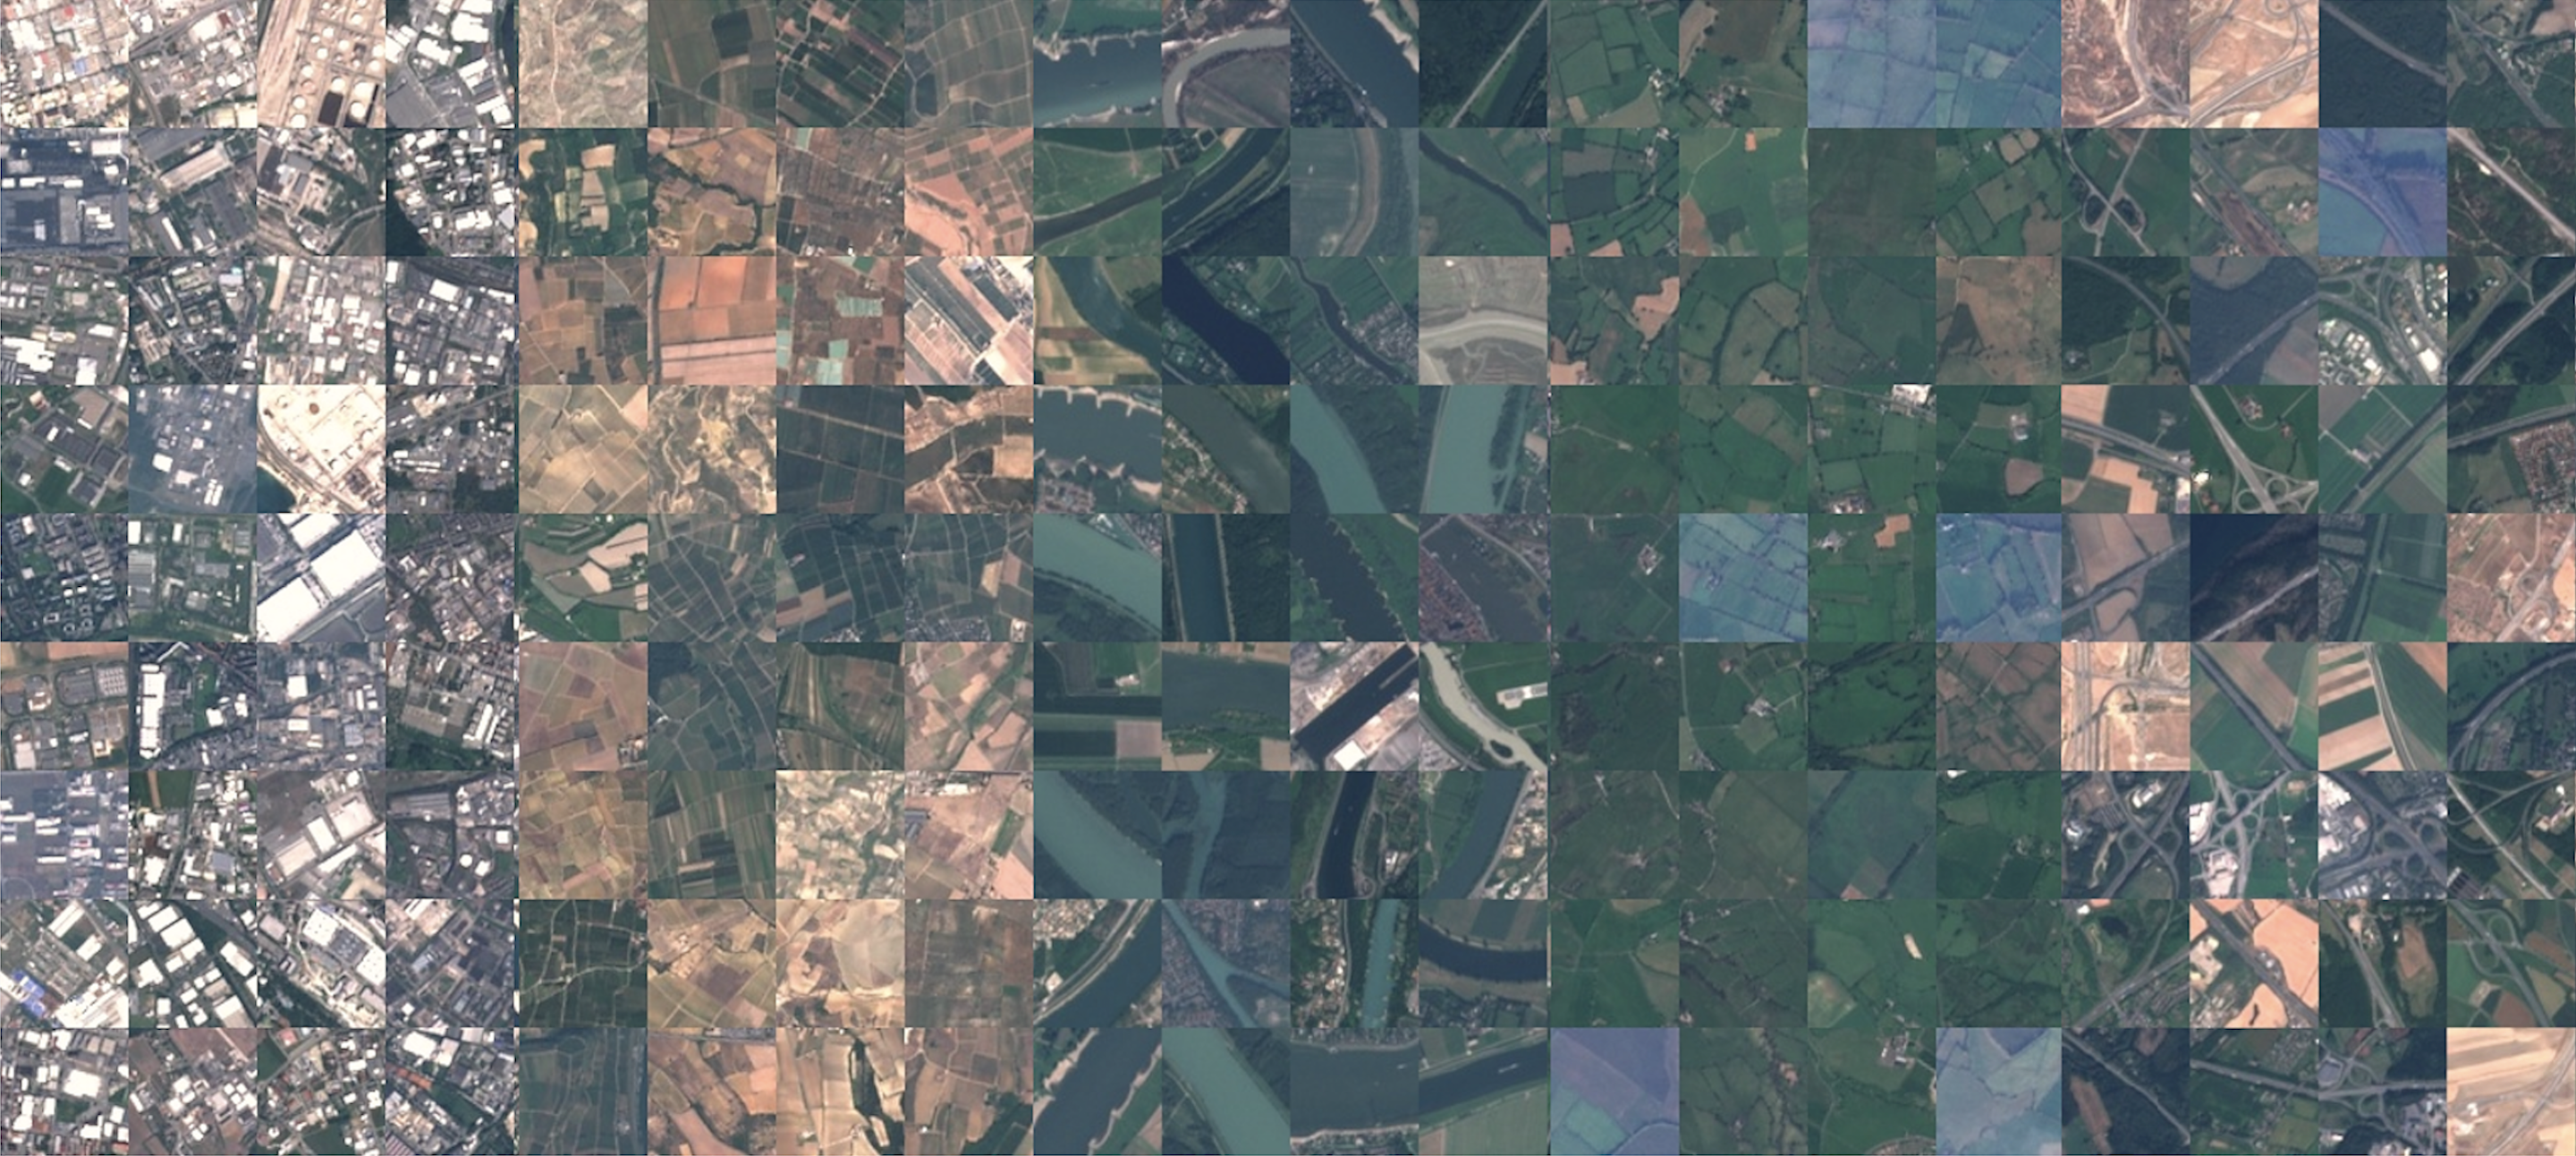
\includegraphics[width=0.8\textwidth]{assets/eurosat-overview.png}
        \caption{Figura adaptada do repositório original\footnote{\href{https://github.com/phelber/EuroSAT/tree/master}{repositório}}.}
        \label{fig:eurosat_samples}
    \end{figure}
\end{frame}

\begin{frame}{Dataset: EuroSAT}
\framesubtitle{1 Introdução - Dados}
    \begin{columns}
        \setlength{\columnsep}{-20cm}
        \begin{column}{0.5\textwidth}
            Detalhes do dataset EuroSAT:
            \begin{itemize}
            \item Imagens de satélite Sentinel-2 da ESA
            \item 27.000 imagens RGB de 64x64 pixels
            \item 10 classes de uso do solo
            \end{itemize}
        \end{column}
        \begin{column}{0.55\textwidth}
            \begin{figure}
                \centering
                \includegraphics[width=\textwidth]{assets/eurosat-classes.png}
                \label{fig:eurosat_classes}
            \end{figure}
        \end{column}
    \end{columns}
\end{frame}

\section{Modelos}

\begin{frame}{MLP (Baseline)}

    \begin{figure}
        \centering
        \includegraphics[width=0.8\textwidth]{assets/mlp_arch.jpg}
        \caption{Arquitetura da MLP.}
        \label{fig:mlp_architecture}
    \end{figure}
\end{frame}

\begin{frame}{VGG-16}

    \begin{figure}
        \centering
        \includegraphics[width=0.8\textwidth]{assets/vgg16-arch.jpg}
        \caption{Arquitetura da VGG-16 \footnote{Figura retirada do \href{https://www.geeksforgeeks.org/computer-vision/vgg-16-cnn-model/}{site}} \cite{vgg16}.}
        \label{fig:vgg16_architecture}
    \end{figure}

\end{frame}

\begin{frame}{ResNet-50}

    \begin{figure}
        \centering
        \includegraphics[width=0.8\textwidth]{assets/resnet_arch.png}
        \caption{Arquitetura da ResNet-50 \cite{resnet50}.}
        \label{fig:resnet50_architecture}
    \end{figure}

\end{frame}

\begin{frame}{Vision Transformer (ViT-B/16)}

    \begin{figure}
        \centering
        \includegraphics[width=0.8\textwidth]{assets/vit_arch.png}
        \caption{Arquitetura do Vision Transformer (ViT-B/16) \cite{vit-b-16}.}
        \label{fig:vit_architecture}
    \end{figure}
\end{frame}

\begin{frame}{Modificações nos Modelos Pré-treinados}
    Nenhuma das arquiteturas pré-treinadas teve suas camadas convolucionais ou de atenção alteradas, apenas as camadas finais foram adaptadas para o problema específico de classificação do EuroSAT. Além disso, todos os modelos pré-treinados tiveram suas camadas base congeladas durante o treinamento inicial, focando o aprendizado nas camadas finais adaptadas.
    \vspace{1em}
    \begin{itemize}
        \item MLP: Nenhuma modificação necessária;
        \item VGG-16: Substituição da camada final do classificador fully connected (FC) para uma camada de Dropout10 e uma FC com 10 saídas (classes da EuroSAT) ;
        \item ResNet-50: Substituição da camada final fully connected para uma FC com 10 classes;
        \item ViT-B/16: Alteração da MLP Head para 10 classes de saída.
    \end{itemize}


\end{frame}

\section{Metodologia}

\begin{frame}{Separação dos Dados}
    \framesubtitle{2 Metodologia - Treino, Validação e Teste}
    \begin{figure}
        \centering
        \includegraphics[width=0.8\textwidth]{assets/metodologia_1.png}
        \caption{Processo de separação dos dados.}
        \label{fig:metodologia_separacao}
    \end{figure}
\end{frame}

\begin{frame}{Separação dos Dados}
    \framesubtitle{2 Metodologia - Treino, Validação e Teste}
        \begin{itemize}
            \item 80\% dos dados para treino e validação (21.600 imagens);
                \item 20\% dos dados para teste (5.400 imagens);
                \item Validação cruzada k-fold estratificado com k=5 para treino e validação.


        \end{itemize}
        \begin{table}[h]
            \centering
            \small
            \caption{Distribuição de imagens por classe em cada fold}
            \label{tab:data_distribution}
            \begin{tabular}{lccccccccccc}
                \hline
                \textbf{Classe} & \textbf{AC} & \textbf{For} & \textbf{HV} & \textbf{Hwy} & \textbf{Ind} & \textbf{Past} & \textbf{PC} & \textbf{Res} & \textbf{Riv} & \textbf{SL} & \textbf{Total} \\
                \hline
                Treino & 1895 & 1934 & 1911 & 1580 & 1612 & 1283 & 1596 & 1915 & 1602 & 1952 & 17280 \\
                Validação & 474 & 484 & 477 & 395 & 404 & 321 & 398 & 479 & 401 & 487 & 4320 \\
                \hline
            \end{tabular}
        \end{table}
\end{frame}
\begin{frame}{Separação dos Dados}
    \framesubtitle{2 Metodologia - Treino, Validação e Teste}
        \begin{figure}
        \centering
        \includegraphics[width=0.8\textwidth]{assets/eurosat-classes-cv.png}
        \caption{Distribuição de imagens por classe em cada fold.}
        \label{fig:data_distribution}
    \end{figure}
\end{frame}


\begin{frame}{Hiperparâmetros e Grid Search}
    \framesubtitle{2 Metodologia - Grid Search e Hiperparâmetros}
    \begin{table}[h]
        \centering
        \tiny
        \caption{Configuração de hiperparâmetros para Grid Search}
        \label{tab:hyperparameters}
        \begin{tabular}{lccccccc}
            \hline
            \textbf{Modelo} & \textbf{Pré-treinado} & \textbf{Weights} & \textbf{Hidden Layers} & \textbf{Dropout} & \textbf{LR} & \textbf{Batch Size} & \textbf{Freeze BB} \\
            \hline
            MLP & Não & - & [512, 256] & 0.3 & 0.001 & 64 & - \\
            \hline
            VGG-16 & Sim & IMAGENET1K\_V1 & - & 0.3 & 0.0001 & 64 & Sim \\
            VGG-16 & Sim & IMAGENET1K\_V1 & - & 0.5 & 0.0001 & 64 & Sim \\
            VGG-16 & Sim & IMAGENET1K\_V1 & - & 0.3 & 0.0001 & 128 & Sim \\
            VGG-16 & Sim & IMAGENET1K\_V1 & - & 0.5 & 0.0001 & 128 & Sim \\
            VGG-16 & Sim & IMAGENET1K\_V1 & - & 0.3 & 0.00001 & 64 & Sim \\
            VGG-16 & Sim & IMAGENET1K\_V1 & - & 0.5 & 0.00001 & 64 & Sim \\
            VGG-16 & Sim & IMAGENET1K\_V1 & - & 0.3 & 0.00001 & 128 & Sim \\
            VGG-16 & Sim & IMAGENET1K\_V1 & - & 0.5 & 0.00001 & 128 & Sim \\
            \hline
            ResNet-50 & Sim & DEFAULT & - & - & 0.0001 & 64 & Sim \\
            ResNet-50 & Sim & DEFAULT & - & - & 0.0001 & 128 & Sim \\
            ResNet-50 & Sim & DEFAULT & - & - & 0.00001 & 64 & Sim \\
            ResNet-50 & Sim & DEFAULT & - & - & 0.00001 & 128 & Sim \\
            \hline
            ViT-B/16 & Sim & IMAGENET1K\_V1 & - & - & 0.00001 & 64 & Sim \\
            \hline
        \end{tabular}
    \end{table}
    \vspace{0.5em}
    \scriptsize
    \textbf{LR}: Learning Rate; \textbf{Freeze BB}: Freeze Backbone
\end{frame}

\begin{frame}{Treinamento dos Modelos}
    \framesubtitle{2 Metodologia - Fluxo de Treinamento}
    \begin{figure}
        \centering
        \includegraphics[width=0.75\textwidth]{assets/training_flow.png}
        \caption{Processo de treinamento dos modelos. (*) Modelos pré-treinados na ImageNet, exceto MLP. (**) Data Augmentation usando RandomFlip, RandomRotation e ColorJitter.}
        \label{fig:training_flow}
    \end{figure}
\end{frame}

\section{Resultados}

\begin{frame}{Resultados dos Treinamento em Validação Cruzada}

    \begin{table}[htbp]
        \centering
        \scriptsize
        % \caption{Model Performance Summary with Mean $\pm$ Standard Deviation}
        \label{tab:model_summary}
        \begin{tabular}{lccccc}
        \hline
            \textbf{Model} & \textbf{Val Acc} & \textbf{Val Loss} & \textbf{Val F1} & \textbf{Val Prec} & \textbf{Val Rec} \\
            \hline
            \textbf{mlp} & $0.3336 \pm 0.0226$ & $1.7809 \pm 0.0489$ & $0.2758 \pm 0.0261$ & $0.3365 \pm 0.0374$ & $0.3336 \pm 0.0226$ \\
            \hline
            \textbf{resnet50} & \textbf{$0.9163 \pm 0.0019$} & \textbf{$0.2888 \pm 0.0034$} & \textbf{$0.9161 \pm 0.0020$} & \textbf{$0.9170 \pm 0.0019$} & \textbf{$0.9163 \pm 0.0019$} \\
            resnet50 & $0.7933 \pm 0.0043$ & $0.9650 \pm 0.0079$ & $0.7914 \pm 0.0038$ & $0.8122 \pm 0.0024$ & $0.7933 \pm 0.0043$ \\
            resnet50 & $0.8281 \pm 0.0011$ & $0.7631 \pm 0.0025$ & $0.8261 \pm 0.0012$ & $0.8365 \pm 0.0009$ & $0.8281 \pm 0.0011$ \\
            resnet50 & $0.9068 \pm 0.0012$ & $0.3310 \pm 0.0019$ & $0.9066 \pm 0.0013$ & $0.9077 \pm 0.0015$ & $0.9068 \pm 0.0012$ \\
            \hline
            vgg16 & $0.9008 \pm 0.0075$ & $0.3774 \pm 0.0278$ & $0.9003 \pm 0.0075$ & $0.9014 \pm 0.0067$ & $0.9008 \pm 0.0075$ \\
            vgg16 & $0.9062 \pm 0.0049$ & $0.2958 \pm 0.0159$ & $0.9058 \pm 0.0049$ & $0.9059 \pm 0.0050$ & $0.9062 \pm 0.0049$ \\
            vgg16 & $0.9748 \pm 0.0031$ & $0.0682 \pm 0.0069$ & $0.9748 \pm 0.0031$ & $0.9752 \pm 0.0029$ & $0.9748 \pm 0.0031$ \\
            \textbf{vgg16} & \textbf{$0.9779 \pm 0.0014$} & \textbf{$0.0640 \pm 0.0028$} & \textbf{$0.9779 \pm 0.0014$} & \textbf{$0.9781 \pm 0.0013$} & \textbf{$0.9779 \pm 0.0014$} \\
            vgg16 & $0.9064 \pm 0.0054$ & $0.3083 \pm 0.0148$ & $0.9060 \pm 0.0053$ & $0.9062 \pm 0.0052$ & $0.9064 \pm 0.0054$ \\
            vgg16 & $0.9004 \pm 0.0057$ & $0.3778 \pm 0.0109$ & $0.8999 \pm 0.0054$ & $0.9004 \pm 0.0052$ & $0.9004 \pm 0.0057$ \\
            vgg16 & $0.9044 \pm 0.0063$ & $0.2994 \pm 0.0153$ & $0.9040 \pm 0.0063$ & $0.9042 \pm 0.0063$ & $0.9044 \pm 0.0063$ \\
            vgg16 & $0.8975 \pm 0.0068$ & $0.4019 \pm 0.0369$ & $0.8973 \pm 0.0068$ & $0.8988 \pm 0.0063$ & $0.8975 \pm 0.0068$ \\
            \hline
            \textbf{vit\_b\_16} & \textbf{$0.9294 \pm 0.0015$} & \textbf{$0.2659 \pm 0.0015$} & \textbf{$0.9295 \pm 0.0015$} & \textbf{$0.9304 \pm 0.0014$} & \textbf{$0.9294 \pm 0.0015$} \\
            \hline
        \end{tabular}
    \end{table}
\end{frame}


\begin{frame}{Resultados dos Treinamento em Validação Cruzada}
    \framesubtitle{4 Resultados - Curvas de Treinamento}

    \begin{figure}
        \centering
        \includegraphics[width=0.8\textwidth]{assets/mlp_best_fold_train.png}
        \caption{Curvas de treinamento do melhor fold da MLP.}
        \label{fig:mlp_train_curve}
    \end{figure}
\end{frame}
\begin{frame}{Resultados dos Treinamento em Validação Cruzada}
    \framesubtitle{4 Resultados - Curvas de Treinamento}

    \begin{figure}
        \centering
        \includegraphics[width=0.8\textwidth]{assets/vgg_best_fold_train.png}
        \caption{Curvas de treinamento do melhor fold da VGG16.}
        \label{fig:vgg_train_curve}
    \end{figure}
\end{frame}
\begin{frame}{Resultados dos Treinamento em Validação Cruzada}
    \framesubtitle{4 Resultados - Curvas de Treinamento}

    \begin{figure}
        \centering
        \includegraphics[width=0.8\textwidth]{assets/resnet_best_fold_train.png}
        \caption{Curvas de treinamento do melhor fold da ResNet50.}
        \label{fig:resnet_train_curve}
    \end{figure}
\end{frame}
\begin{frame}{Resultados dos Treinamento em Validação Cruzada}
    \framesubtitle{4 Resultados - Curvas de Treinamento}

    \begin{figure}
        \centering
        \includegraphics[width=0.8\textwidth]{assets/vit_best_fold_train.png}
        \caption{Curvas de treinamento do melhor fold da ViT-B/16.}
        \label{fig:vit_train_curve}
    \end{figure}
\end{frame}

\begin{frame}{Resultados Finais no Conjunto de Teste}
    \framesubtitle{4 Resultados - Teste}

    \begin{table}[htbp]
    \centering
    \caption{Acurácias Finais no Conjunto de Teste}
    \label{tab:test_results}
        \begin{tabular}{lc}
            \hline
            \textbf{Model} & \textbf{Accuracy} \\
            \hline
            ViT-B/16 & 0.9405 \\
            \textbf{VGG-16} & \textbf{0.9439}\\
            ResNet50 & 0.9131 \\
            MLP & 0.2041 \\
            \hline
        \end{tabular}
    \end{table}

\end{frame}

\begin{frame}{Resultados Finais no Conjunto de Teste}
    \framesubtitle{4 Resultados - Teste - ViT-B/16}


            \begin{figure}
                \centering
                \includegraphics[width=0.55\textwidth]{assets/vit_cm.png}
                \scriptsize
                \caption{Matriz de Confusão do ViT-B/16 no conjunto de teste.}
                \label{fig:vit_confusion_matrix}
            \end{figure}


\end{frame}


\begin{frame}{Resultados Finais no Conjunto de Teste}
    \framesubtitle{4 Resultados - Teste - VGG-16}


            \begin{figure}
                \centering
                \includegraphics[width=0.55\textwidth]{assets/vgg_cm.png}
                \scriptsize
                \caption{Matriz de Confusão do VGG-16 no conjunto de teste.}
                \label{fig:vgg_16_confusion_matrix}
            \end{figure}


\end{frame}
\begin{frame}{Resultados Finais no Conjunto de Teste}
    \framesubtitle{4 Resultados - Teste - ResNet-50}


            \begin{figure}
                \centering
                \includegraphics[width=0.55\textwidth]{assets/resnet_cm.png}
                \scriptsize
                \caption{Matriz de Confusão do ResNet-50 no conjunto de teste.}
                \label{fig:resnet_50_confusion_matrix}
            \end{figure}


\end{frame}
\begin{frame}{Resultados Finais no Conjunto de Teste}
    \framesubtitle{4 Resultados - Teste - MLP}


            \begin{figure}
                \centering
                \includegraphics[width=0.55\textwidth]{assets/mlp_cm.png}
                \scriptsize
                \caption{Matriz de Confusão do MLP no conjunto de teste.}
                \label{fig:mlp_confusion_matrix}
            \end{figure}


\end{frame}

\section{Conclusão}

\begin{frame}{Conclusão}
    \begin{itemize}
        \item A VGG-16 obteve o melhor desempenho no conjunto de teste, seguida pelo ViT-B/16 e ResNet-50.
        \item A MLP teve um desempenho significativamente inferior, destacando a importância de arquiteturas mais complexas para tarefas de visão computacional.
        \item Redes convolucionais tradicionais ainda são altamente eficazes para classificação de imagens, apesar do avanço dos Transformers.
        \item Futuras pesquisas podem explorar outras arquiteturas e técnicas de pré-processamento para melhorar ainda mais o desempenho.
    \end{itemize}
\end{frame}

\section{Referências Bibliográficas}
\begin{frame}[allowframebreaks]
        \frametitle{Referências Bibliográficas}
        \bibliographystyle{ieeetr}
        \bibliography{presentation_bib.bib}
\end{frame}

\backmatter
\end{document}
